% TEMPLATE for Usenix papers, specifically to meet requirements of
%  USENIX '05
% originally a template for producing IEEE-format articles using LaTeX.
%   written by Matthew Ward, CS Department, Worcester Polytechnic Institute.
% adapted by David Beazley for his excellent SWIG paper in Proceedings,
%   Tcl 96
% turned into a smartass generic template by De Clarke, with thanks to
%   both the above pioneers
% use at your own risk.  Complaints to /dev/null.
% make it two column with no page numbering, default is 10 point

% Munged by Fred Douglis <douglis@research.att.com> 10/97 to separate
% the .sty file from the LaTeX source template, so that people can
% more easily include the .sty file into an existing document.  Also
% changed to more closely follow the style guidelines as represented
% by the Word sample file. 

% Note that since 2010, USENIX does not require endnotes. If you want
% foot of page notes, don't include the endnotes package in the 
% usepackage command, below.

\documentclass[letterpaper,twocolumn,10pt]{article}
\usepackage{usenix,epsfig,endnotes,comment}
\begin{document}

%don't want date printed
\date{}

%make title bold and 14 pt font (Latex default is non-bold, 16 pt)
\title{\Large \bf Data assimilation for ABMs}

\author{
{\rm Daniel Tang}\\
Oxford University
}

\maketitle

% Use the following at camera-ready time to suppress page numbers.
% Comment it out when you first submit the paper for review.
%\thispagestyle{empty}


\subsection*{Abstract}

We show how to go about doing data assimilation on ABMs.

\section{Introduction}

The problem of interest here is as follows: suppose we have some observations of a real-world complex system, $Y=(y_0...y_T)$, and a computer model of the system, $\theta_{t+1} = \Phi(\theta_t)$; how do we get information about the probability distribution over the parameters and initial state of the model given the observations, $P(\theta_0|Y)$? In particular, we would like to find the most probable $\theta_0$, known as the `analysis`, and some quantification of the uncertainty in $\theta_0$.

On the surface of it, finding the mode of $P(\theta_0|Y)$ is just a case of using non-linear optimisation to maximise the probability. Using Bayes, we can express the function to be maximised as
\[
P(\theta_0|Y) = \frac{P(Y|\theta_0)P(\theta_0)}{P(Y)}
\]
but since $P(Y)$ is independent of $\theta_0$ we only need to maximise  $P(Y|\theta_0)P(\theta_0)$, or more conveniently, $\ln(P(Y|\theta_0))+\ln(P(\theta_0))$ where
\[
\ln{(P(Y|\theta_0))} = \sum_t{\ln{(P(y_t|\Phi^t(\theta_0)))}}
\]

As is generally the case in non-linear optimisation, there is no one-size-fits-all technique to perform this optimisation. Instead we will explore classes of systems that present difficulties and provide ways to optimise these. We will then present rules to decide whether a given system is within a difficult class. Ultimately these can be coded into an automated tool that can identify which class a given system belongs to and apply the appropriate technique to optimise it. To the extent that there remains some trial-and-error, the algorithm can automatically search the space of possible optimisation strategies. In this way we take as much of the menial effort as possible away from the user.

It is worth splitting the problem into two: The first is the problem of maintaining the data assimilation cycle; that is, given a prior from the previous assimilation cycle and a set of new observations how do we calculate the analysis and the prior for the next assimilation cycle. The success of the solution can be judged by the set of observations for which the uncertainty remains small (or at least bounded). The second is the problem of getting the data assimilation cycle started in the first place. In this case, the prior may be much wider than it is once the assimilation cycle gets started and may encompass many local minima, so the problem is potentially harder.

A good solution to the second problem is likely to also be a good solution to the first, however, we may be able to find a computationally more efficient solution to the first that would not be applicable to the second.

\section{Chaotic Systems, e.g. Lorenz '63}

Chaotic systems present a difficulty to optimisation because their sensitive dependence to initial conditions can lead to very large rates of change of the objective function, and many local minima. To illustrate this, consider the Lorenz equations (1963). Suppose we observe only the X co-ordinate over a 10,000 time-step integration ($\Delta t=0.01$) starting at some random point on the attractor $(0.66978, -3.57054, 26.4651)$. Suppose also that $P(x|\theta)$, the probability of making observation $x$ in state $\theta=(\theta_x,\theta_y,\theta_z)$, is Gaussian so $ln(P(x|\theta)) \propto -(x-\theta_x)^2$. We wish to optimise over the initial state $\theta_0$, but since the x component of this is observed, we only need to vary the y and z components. Figure \ref{noNudging} shows the objective function for the $y$ and $z$ values of $\theta_0$ around the correct solution. There are many local maxima and standard optimisation algorithms would not find the correct solution unless the error in the initial guess was very small indeed.

\begin{figure}
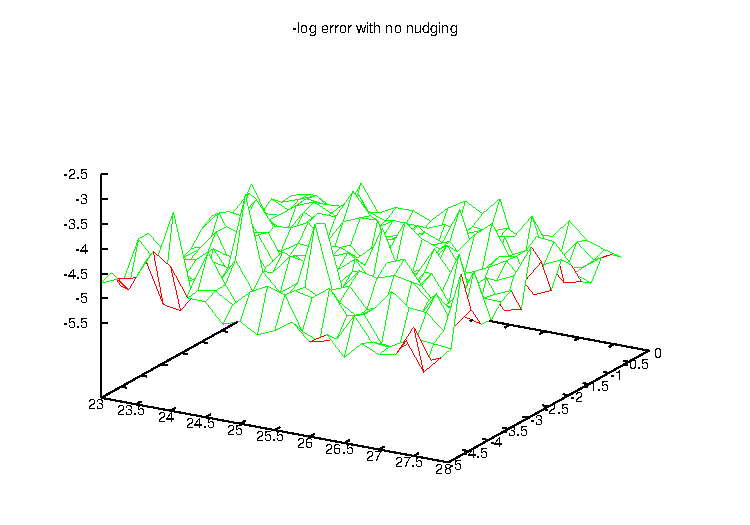
\includegraphics[width=0.48\textwidth]{rawOut.pdf}
\caption{Minus the log of the squared error between observations and simulated observations with no nudging for various start values of Y and Z, for a 10,000 timestep observation window. The correct solution is (-3.57, 26.47)}
\label{noNudging}
\end{figure}

The problem occurs because small errors in $\theta_0$ quickly amplify until the state of the simulation bears no relation to the state of the observed system. This can quite easily be fixed by ``nudging`` the system towards the observations at each time-step (in this case, by updating the x coordinate according to $\theta'_{x}=0.6\theta_x + 0.4x$, where $x$ is the observation. Nudging is a technique often used when embedding a high resolution fluid dynamical model inside a larger, lower resolution model). This nudging can be considered in many different ways, but the most mathematically consistent interpretation is to consider that there is a Gaussian noise in both the observation and the model time-step. The nudged value then gives us the most probable underlying model state that would give rise to both the observation and the noisy model output.

Figure \ref{withNudging} shows the objective function around the correct solution in the presence of nudging. This function can be optimised by standard non-linear optimisation algorithms to find the correct solution.

\begin{figure}
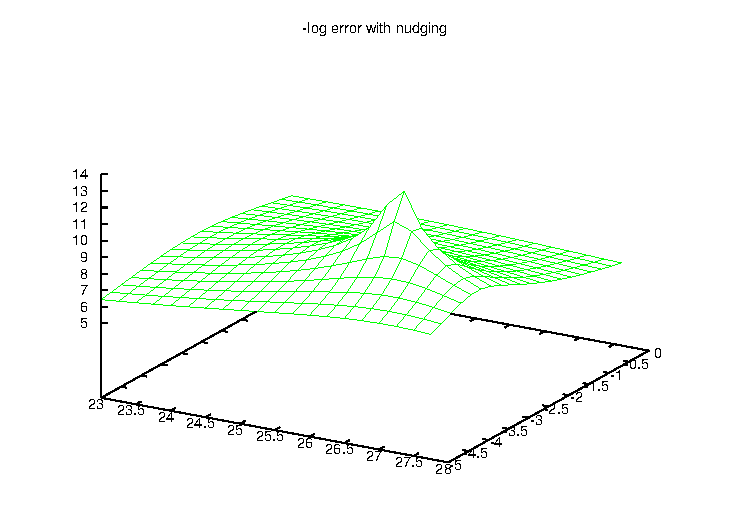
\includegraphics[width=0.48\textwidth]{nudgingOut.pdf}
\caption{Minus the log of the squared error between observations and simulated observations with nudging for various start values of Y and Z, for a 10,000 timestep observation window}
\label{withNudging}
\end{figure}

\section{Systems with many discontinuities}

In discrete systems, we may have many discontinuities in the objective function. For example, if we are considering the prevalence of an infectious disease in a finite population, changes in the proportion infected would change in finite steps, and if this is one of the observables these may translate into finite steps in the objective function. In this case, the analytical rate of change of the objective function with the initial state may be zero almost everywhere, making optimisation algorithms that use automatic differentiation ineffective (and these are the only ones we can use when the state space is very large).

In order to deal with this problem, we add some kind of random draw to the model and marginalise over that draw.

In the case of agent based models, we present the following very general solution: We restrict ourselves to the consideration of sets of $N$ agents whose internal states, $(\sigma_0...\sigma_N)$, are drawn from a smooth distribution, $P_\psi(\sigma)$, where $\psi$ is some parameterisation of the distribution. For a given $\psi$ there is a probability distribution over the actual agent states, $\theta_0$, that are drawn from $P_\psi$. The function $P(Y|\psi, ... )$ is now smooth, even if $P(Y|\theta_0)$ isn't, since we're marginalising over a smooth PDF $P(Y|\psi, ... ) = \int_{\theta_0} P_\psi(\theta_0)P(Y|\theta_0, ... )$.

We can calculate (or at least approximate) the marginalisation integral by Monte-Carlo simulation, and given this we can calculate the differentials $\frac{\partial P(Y|\psi,...)}{\partial \psi}$ by holding the Monte-Carlo runs fixed so that we only need to calculate $\frac{dP_\psi(\theta_0)}{d\psi}$ which are already known. These can then be fed into a standard non-linear optimiser. At each iteration of the optimisation another set of Monte-Carlo runs will be made. When drawing model states for the Monte Carlo simulations, it may increase the stability of the optimisation to have the states vary smoothly with changes in $\psi$ rather than taking a completely new random draw at each iteration.

[Continue with SIR model, then with chaotic, two strain SIR]

\begin{comment}
rough notes
-----------
There are three ways of looking at an ABM:

As a computer program with inputs and outputs where the inputs consist of the parameters and initial conditions, $\theta$, which we will call the initial state, while the output, in the case of data assimilation, is the posterior $P(\theta|y)$, the probability (density) that $\theta$ are the true parameters and start state given that we made observations $y$, or, more practically, $\ln(P(y|\theta)P(\theta))$.

As a probabilistic computer program whose inputs are the initial state, and whose output is a set of observations of the system (i.e. the set of observations that we have).

When thinking about computer programs, we define the trace of the program to be the vector of memory states the computer is in as it passes a set of trace points (usually, the start of a time-step).

As a continuous dynamic system whose state space spans the memory states of the ABM, whose trajectories for a given start state pass through the memory states in the trace. Since we do not specify what happens between time-steps this is a one-many mapping.

As a posterior PDF: a map from inputs (parameters and start state) to outputs (posterior probability).

Given a prior over the model states $P(\theta)$, it is usually easy to write a program to calculate the log posterior to within a constant. This posterior will generally have quite a complex form, our aim in data assimilation is to find out various properties of this PDF.

Likely things we may want to find: point estimates such as the mode or the mean, the variance, percentiles, best fit to some family of PDFs.



\subsection{Defining discontinuity}

Strictly speaking, since any computer program with finite space complexity has a finite number of discrete states, there always exists a smooth dynamic system whose trajectories pass through the discrete trajectories of the computer program. However, if the rate of change in the trajectory approaches that of the reciprocal of the precision of the inputs, then we consider this a discontinuity. If the trajectory is discontinuous in the inputs, this discontinuity may cause a discontinuity in the posterior.

This is a problem for optimisation algorithms, not so much because we may land on a discontinuity, but more because a better solution can hide behind a discontinuity.

One way to deal with this is, rather than deal with points in the initial state space we deal with a PDF in the initial state space with a support $\Theta$ and a probability $P_\Theta(\theta)$. That is, rather than calculate $\ln(P(y|\theta)P(\theta))$ we calculate
\[
\ln\left(\int_{\theta\in\Theta} P(y|\theta)P(\theta)P_{\Theta}(\theta) \right)
\]
If we let $P_\Theta(\theta) = P_k(\theta - \psi)$ for some kernel $P_k$ then we end up with a PDF in $\psi$ which is a convolved, or blurred, and continuous, version of the original, discontinuous PDF.

This is particularly useful since we can control the amount of blurring, solving first for high blurring then iteratively solving while the blurring is reduced.

How do we perform automatic differentiation on a PDF of initial states? Sampling will generally not work (or will it?) Since we don't much care about the exact form of $P_k$,

We could turn \texttt{if} statements into probabilistic conditionals (i.e the body of the if statement is executed probabilistically according to a sigmoid). However, this could result in execution paths that are impossible in the deterministic limit.

We could add noise to the state at the end of each time-step.

We could do automatic integration

We could combine information about probability density and rate of change at a number of sample points taken from $\Theta$, to give a best estimate.

We could use the Chebyshev approximation of the model on $\Theta$ and integrate that. Constructing the Chebyshev integration should be done in reverse mode, adding terms to the log probability as we move back through observations.

We should choose a $\Theta$ carefully so that the volume of trajectories remains small. That is, $\Theta$ should be thin in the directions where the Lyapunov exponent is greater than 1, and the end state should be thin in the directions where the Lyapunov exponent is less than one. This can be done by dynamically scaling the Chebyshev tangent model.

We could MCMC sample and just choose the sample that has the highest probability.

We could restrict ourselves to sets of agents drawn from a smooth distribution, and restrict observables to probability of observing a given behaviour (when integrated over an infinite number of draws from the distribution). Whenever an agent's behaviour is discontinuous in the initial state, we define a smooth heterogeneity of agents in the set that has the effect of smoothing the observable.

Suppose a set of agents consists of a PDF over internal states of those agents and a cardinality of the set (possibly infinite). We can define the dynamics of such a set by defining the conditional probability of an autonomous change of state $P(x'|x)$. All interaction between agents occurs as message passing where a given change of state is associated with the emmission of a given message. On receipt of a message, an agent changed state to one associated with that message being in its `inbox'.

The PDF will become very complex, but can be represented as a probabilistic program If each step consists of choosing an agent from the PDF and performing a single transition, then in the backwards mode we can analytically integrate over the choice of agent. (or, perhaps we can do a separate transformation of the program beforehand by analytically integrating once and for all - over the whole input space - then sending for data assimilation).
\end{comment}


%{\footnotesize \bibliographystyle{acm}
%\bibliography{sample}}


%\theendnotes

\end{document}
